\section{Methodology} \label{sec:Methodology}

\subsection{Notation}

In this manuscript, we define three reference frames. $W$ is the fixed world frame, whose $z$ axis is aligned with the gravity, $B$ is the quadrotor body frame, and $C$ is the camera frame. These reference frames are depicted in Fig.~\ref{fig:reference_frames}. We represent vectors and matrices as bold quantities. We use capital letters for matrices. Vectors have a suffix representing the frame in which they are expressed and their endpoint. For example, the quantity $\bm{p}_{WB}$ represents the position of the body frame $B$ with respect to the world frame $W$. We use the symbol $\bm{R}_{WB}$ to denote the rotation matrix that rotates a vector from the frame $B$ to the frame $W$. We use $\bm{q}_{WB}$ to denote the quaternion representation of this rotation. The time derivative of a vector $\bm{v}$ is represented by $\dot{\bm{v}}$. In the case of quaternion, the time derivative is defined as $\dot{\bm{q}} = \frac{1}{2} \Lambda (\bm{\omega})$, where $\Lambda(\bm{\omega})$ is the screw-symmetric matrix of the vector $\bm{\omega}$. The symbol $\odot$ represents the quaternion-vector product. The symbol $\times$ represents the cross product between two vectors.

\subsection{Quadrotor Dynamics}
\begin{figure}[t!]
    \centering
    \tdplotsetmaincoords{65}{30}
\begin{tikzpicture}[tdplot_main_coords, >=latex]
\tikzset{RPY/.style={x={(\nxx,\nxy)},y={(\nyx,\nyy)},z={(\nzx,\nzy)}}}
\def\propz{0.5}
\def\propx{2.4}
\def\propy{2.2}
\def\r{1}
\def\l{1.2}
\def\f{0.8}
\def\c{0.8}
\def\x{0}
\rotateRPY{-10}{20}{0}
\begin{scope}[RPY]
% frame
\draw[] (-\propx-\x,0,0) -- (\propx-\x,0,0);
\draw[] (-\x,-\propy,0) -- (-\x,\propy,0);
% rotors
\draw[draw=none, fill=black, opacity=0.15] (0-\x,\propy,\propz) circle (\r);
\draw[draw=none, fill=black, opacity=0.15] (\propx-\x,0,\propz) circle (\r) ;
\draw[draw=none, fill=black, opacity=0.15] (0-\x,-\propy,\propz) circle (\r) ;
\draw[draw=none, fill=black, opacity=0.15] (-\propx-\x,0,\propz) circle (\r) ;
\draw (-\x,\propy,0) --++ (0,0,\propz) node[right] {4};
\draw (\propx -\x,0,0) --++ (0,0,\propz) node[right] {2};
\draw (-\x,-\propy,0) --++ (0,0,\propz) node[right] {1};
\draw (-\propx -\x,0,0) --++ (0,0,\propz) node[left] {3};
% forces
\draw[thick,->] (-\x,\propy,\propz) -- ++(0,0,\f);
\draw[thick,->] (\propx-\x,0,\propz) -- ++(0,0,\f);
\draw[thick,->] (-\x,-\propy,\propz) -- ++(0,0,\f);
\draw[thick,->] (-\propx-\x,0,\propz) -- ++(0,0,\f);    

% propeller rotation
\def\psi{60}
\def\xa{30}
\def\xb{0}
\def\xc{-90}
\def\xd{210}
\path (\r-\x,\propy,\propz) arc (0:\xa:\r) coordinate (a);
\draw [->] (a) arc (\xa:\xa-\psi:\r) [draw=black] ;
\path (\propx-\x,\r,\propz) arc (90:\xb:\r) coordinate (b);
\draw [->] (b) arc (\xb:\xb+\psi:\r) [draw=black] ;
\path (\r-\x,-\propy,\propz) arc (0:\xc:\r) coordinate (c);
\draw [->] (c) arc (\xc:\xc-\psi:\r) [draw=black] ;
\path (-\propx-\x,\r,\propz)  arc (90:\xd:\r) coordinate (d);
\draw [->] (d) arc (\xd:\xd+\psi:\r) [draw=black] ;
% quad frame
\rotateRPY{0}{0}{45}
\begin{scope}[RPY]
\draw[->,color=red,text=black] (-\x,0,0) -- ++ (\l,0,0) node[above] {$\bm x_\bfr$};
\draw[->,color=green,text=black] (-\x,0,0) -- ++ (0,\l,0) node[above] {$\bm y_\bfr$};  
\draw[->,color=blue,text=black] (-\x,0,0) -- ++ (0,0,\l) node[left] {$\bm z_\bfr$};     
\rotateRPY{0}{25}{0}

% camera frame
\begin{scope}[RPY, xshift=3.5cm, yshift=-0.75cm]
\draw[->,color=red,text=black] (-\x,0,0) -- ++ (\l,0,0) node[left=1] {$\bm x_C$};
\draw[->,color=green,text=black](-\x,0,0) -- ++ (0,\l,0) node[above] {$\bm y_C$};  
\draw[->,color=blue,text=black] (-\x,0,0) -- ++ (0,0,\l) node[left=1] {$\bm z_C$}; 
\end{scope}

%draw the angle arc
\draw[densely dotted](4.6,0,0) arc (0:-45:0.8) node[right=3] {$30^{\circ}$};

% connect center of body and camera
\draw[dotted]{(0, 0, 0) --++ (5.3, 0, 0)};

\end{scope}
\end{scope}

% world frame
\begin{scope}[xshift=-3cm, yshift=-2cm]
\draw[->,color=red,text=black] (-\x,0,0) -- ++ (\l,0,0) node[right] {$\bm x_\wfr$};
\draw[->,color=green,text=black] (-\x,0,0) -- ++ (0,\l,0) node[above] {$\bm y_\wfr$};  
\draw[->,color=blue,text=black] (-\x,0,0) -- ++ (0,0,\l) node[left] {$\bm z_\wfr$};

% draw a power line
\draw[->]{(0, 0, -1) --++ (8.5, 0, 0)} node[right=3]{};
\node at (5.5, 0, -0.25) [canvas is xz plane at y=0] {Power line detection};

% draw two points
\rotateRPY{0}{0}{0}
\draw[fill=black](1, 0, -1) circle (0.15) node[below=2] {$\bm{p}_{WL_1}$};
\draw[fill=black](7.5, 0, -1) circle (0.15) node[below=2] {$\bm{p}_{WL_2}$};
\end{scope}
\draw{(0, 0, -3.32+0.2-0.7) --++ (0.2, 0, 0)};
\draw{(0.2, 0, -3.32+0.2-0.7) --++ (0, 0, -0.2)};
\draw[dotted]{(0, 0, 0) --++ (0, 0, -4)};
\draw[thick,->,color=black,text=black] (-\x,0,0) -- node[below right] {$\bm g_\wfr$} ++ (0,0,-2*\f);

% Yaw
% \draw[thin,->] (-1.0,-1,-0.5) arc (0:45:0.5) node[midway, right] {$\heading$};
% gravity
\end{tikzpicture}
    \caption{Diagram of quadrotor and power line model.}
    \label{fig:reference_frames}
    \vspace{-1.5ex}
\end{figure}

Let $\bm{p}_{WB}$, $\bm{q}_{WB}$ and $\bm{v}_{WB}$ be the position, orientation, and linear velocity of the quadrotor expressed in the world frame $W$. Let $\bm{\omega}_{B}$ be the angular velocity of the body expressed in the body frame $B$.
Additionally, let $c = \Sigma_i c_i$ be the body collective thrust, where $c_i$ is the thrust produced by the i-th motor, $\bm{c} = \begin{bmatrix} 0,  0, c\end{bmatrix}^\intercal$ be the collective thrust vector, $m$ be the mass of the quadrotor, and $\bm{g}_W$ be the gravity vector.
Finally, let $\bm{J}$ be the diagonal moment of inertia matrix and $\bm{\tau}_B$ the body collective torque. The quadrotor dynamical model is:
%
\begin{equation}
	\begin{aligned}
		\dot{\bm{x}} = \begin{bmatrix}
			\dot{\bm{p}}_{WB} \\
			\dot{\bm{q}}_{WB} \\
			\dot{\bm{v}}_{WB} \\
			\dot{\bm{\omega}}_{B} \\
		\end{bmatrix} = \begin{bmatrix}
		\bm{v}_{WB}\\
		\frac{1}{2} \Lambda({\omega}_B) \cdot \bm{q}_{WB}\\
		\bm{q}_{WB} \odot \bm{c}/m + \bm{g}_W\\
		\bm{J}^{-1}(\bm{\tau}_B - \bm{\omega}_B\times \bm{J} \cdot \bm{\omega}_B)
	\end{bmatrix}
	\end{aligned}\label{eq:dynamics}
\end{equation}
%
The body torque $\bm{\tau}_B$ is represented by:
\begin{equation}
	\bm{\tau}_B = \begin{bmatrix}
		-d_{x_0}&-d_{x_1}&d_{x_2}&d_{x_3}\\
		d_{y_0}&-d_{y_1}&-d_{y_2}&d_{y_3}\\
		-c_{\tau}&c_{\tau}&-c_{\tau}&c_{\tau}
	\end{bmatrix}\begin{bmatrix}
		c_1\\c_2\\c_3\\c_4
	\end{bmatrix}
\end{equation}
where $d_{x_i}$, $d_{y_i}$ for $i$ = [1, 2, 3, 4] are the distances of each rotor $i$ to the body frame and $c_\tau$ is the rotor drag constant. The state and input vector of the system are $\bm{x} = [\bm{p}_{WB}^\intercal, \bm{q}_{WB}^\intercal, \bm{v}_{WB}^\intercal, \bm{w}_{B}^\intercal]^\intercal$ and  $\bm{u} = [c , \bm{\omega}_B^\intercal]^\intercal$.

\subsection{MPC Formulation}\label{ch2_mpc}
%
The system dynamics in Eq.~\ref{eq:dynamics} can be written in compact form as $\dot{\bm{x}} = f(\bm{x}, \bm{u})$. We compute the discrete-time version of it by using a Runge-Kutta method of 4th order with time step $dt$: $\bm{x}_{i+1} = f(\bm{x}_i, \bm{u}_i, dt)$. The MPC formulation is a non-linear program with quadratic costs:
%
\begin{equation}
	\begin{aligned}
		\mathcal{L}_{org} =\, &\bar{\bm{x}}_N^\intercal \mathcal{Q}_{x,N} \bar{\bm{x}}_N ~+ \sum_{i=0}^{N-1} \left(\bar{\bm{x}}_i^\intercal \mathcal{Q}_{x} \bar{\bm{x}}_i + \bar{\bm{u}}_i^\intercal \mathcal{R} \bar{\bm{u}}_i\right) \\
		& \argmin_{\bm{u}} \; \mathcal{L}_{org} \\
		& \text{s.t.} 
		\begin{array}[t]{l}
			\bar{\bm{x}}_0 = \bm{x}_{init}\\
			\bm{x}_{i+1} = f(\bm{x}_i, \bm{u}_i)\\
        \bm{u}_{\textrm{min}} \leq  \bm{u}_i\leq\bm{u}_{\textrm{max}}.
		\end{array}
	\end{aligned}\label{eq:classical_mpc}
\end{equation}
%
This is solved as a sequential quadratic program (SQP) executed in a real-time iteration scheme~\cite{diehl2006fast}. The values $\bar{\bm{x}} = \bm{x} - \bm{x}_s$ and $\bar{\bm{u}} = \bm{u} - \bm{u}_s$ refer to the difference with respect to the reference of each value. We implement this optimization problem in ACADO~\cite{houska2011acado} and use the qpOASES solver~\cite{ferreau2014qpoases}.
\begin{figure}
	\centering
	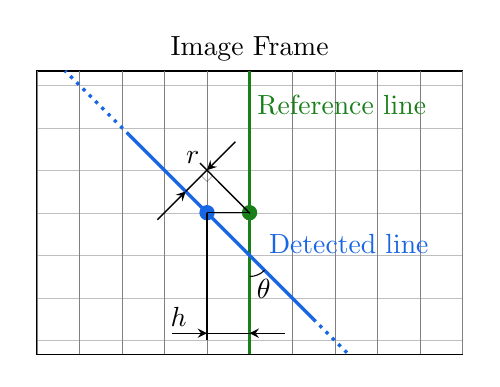
\begin{tikzpicture}[x=0.018cm,y=0.018cm]
\definecolor{my_green}{rgb}{0.1, 0.5, 0.1}
\definecolor{my_blue}{rgb}{0.1, 0.4, 0.9}


% Rectangle
\node (rect) at (0, 0) [draw, minimum width=5.4cm, minimum height=3.6cm] {};
\draw [] (rect) node[above, yshift=1.8cm] {Image Frame};
\foreach \i in {-5 ,...,5} {
        \draw [line width=0.05,gray] (\i * 30, -100) -- (\i * 30,100)  node [below] at (\i * 30,100) {};
        }

\foreach \i in {-3 ,...,3} {
    \draw [line width=0.05,gray, opacity=0.5] (-150, \i * 30) -- (150, \i * 30)  node [below] at (150, \i * 30) {};}
% Green middle line
\draw [color=my_green, line width=1.2] (0, -100) -- (0, 100) ;

% Blue middle line
\draw [color=my_blue, line width=1.2][fill={rgb, 255:red, 65; green, 117; blue, 5 }  ,fill opacity=1 ]   (100 - 5*11, -100 + 5 * 11 - 30) -- (-100 + 5*3, 100 - 5 * 3 - 30) ;

%  Center circles
\draw [color=my_green, fill=my_green](0, 0) circle (5) ;
\draw [color=my_blue, fill=my_blue] (-30, -0) circle (5) ;

% Blue dashed line
\draw [dotted][color=my_blue, line width=1.2] (100 - 5 * 11, -100 + 5 * 11  - 30) -- (70, -100) ;

\draw [dotted][color=my_blue, line width=1.2](-100 + 5*3, 100 - 5*3 - 30) -- (-130, 100) ;

% Connect two center circles
\draw [line width=0.5](0.25, -0.5) -- (-35, 35) ;

% Connect two center points
\draw [line width=0.5](-30, -0) -- (0, 0);

% Draw arrows
\draw [line width=0.5][stealth-](-30, 30) -- (-30 + 20,  30 + 20);
\draw [line width=0.5][stealth-](-45, 15) -- (-45 - 20, 15 - 20);

% Connect two arrows
\draw [line width=0.5](-30, 30) -- (-45, 15);
% Perpendicular symbol
\draw [line width=0.1](-30 + 4, 30 - 4) -- (-30, 30 - 8);
\draw [line width=0.1](-30 - 4, 30 - 4) -- (-30, 30 - 8);

% Draw vertical line
\draw [line width=0.5](-30, 0) -- (-30, -10 - 80);
\draw [line width=0.5][stealth-](0, -10 - 80  +5 ) -- (0 + 25, - 10 - 80 + 5); 
\draw [line width=0.5][stealth-](-30, -10-80  +5 ) -- (-30 - 25, -10-80 + 5); 
\draw [line width=0.5](-30, -10-80 + 5) -- (0, -10-80 + 5);

%Draw angle arc
\draw (0,-45) arc (270:315:15);

% Draw texts
\draw [color=my_green] (65, 90) node[below] {Reference line};
\draw [color=my_blue] (70, -8) node[below] {Detected line};
\draw (-40, 50) node[below] {$r$};
\draw (-50, -60) node[below] {$h$};
\draw (10, -40) node[below] {$\theta$};




\end{tikzpicture}
	\vspace{0.5ex}
	\caption{Illustration of a reference and detected line onto the image frame.}
	\vspace{-1.5ex}
	\label{fig:lineeval}
\end{figure}

\subsection{Perception Objectives}\label{ch2_perception}
We include two perception objectives: one for line tracking and one for collision avoidance, in the MPC formulation proposed in Eq.~\ref{eq:classical_mpc}.

\medskip
\textbf{Line Tracking: }
The purpose of this objective is to keep the power line in the center of the image (c.f. Fig.~\ref{fig:lineeval}), to maximize data quality for visual inspection, \iros{and to keep a safe distance from the power lines}. We derive the line tracking objective in this section by extending the perception objective proposed for a single point in~\cite{Falanga18iros}. We denote the position of the line endpoints in the world frame $W$ as $\bm{p}_{W{L_j}} \; j\in\left\{1, 2\right\}$. These points are transformed to the camera frame $C$ by:
\begin{equation}
	\bm{p}_{C{L_j}} = (\bm{q}_{WB} \cdot \bm{q}_{BC})^{-1} \odot (\bm{p}_{W{L_j}} - (\bm{q}_{WB} \odot \bm{p}_{BC} + \bm{p}_{WB}).
	\label{eq:line_endpoints_camera_frame}	
\end{equation}
The points: $\bm{p}_{C{L_1}}$ and $\bm{p}_{C{L_2}}$ are projected into the image plane coordinates: $[u_1, v_1], [u_2, v_2]$ according to the classical pinhole camera model~\cite{Szeliski10book}. The cartesian coordinates are transformed into the polar coordinates as:
\begin{equation}\label{eq:cartesian_to_polar}
		\theta = \arctan\left(-\frac{u_2 - u_1}{v_2 - {v_1}}\right), \;
		r = \left(v_1 - \frac{v_2 - v_1}{u_2 - u_1} u_1 \right) \sin\theta.
\end{equation}
We introduce a new variable $\bar{\bm{z}}$ in our MPC formulation:
\begin{equation}
	\bm{z} = \left(\begin{array}{c}
		\theta \\
		r \\
		d
	\end{array} \right), \qquad
	\bm{z}_s = \left(\begin{array}{c}
		0 \\
		0 \\
		d_s
	\end{array} \right), \qquad
	\overline{\bm{z}} = \bm{z} - \bm{z}_s.
\end{equation}

The variable $d$ represents the distance of the line to the body frame (c.f. Fig.~\ref{fig:reference_frames}) and $d_s$ represents the \iros{target} value of $d$. \iros{The value of $d_s$ is set by the user according to the desired distance of the flight from the power lines.}
\medskip
\textbf{Obstacle Avoidance:}
Inspired by~\cite{zhu2019chance,lin2020robust}, we include collision avoidance capabilities in our MPC by means of a collision cost and a collision constraint. The collision cost $l_{o}$ is formulated with the logistic function:
%
\begin{equation}\label{eq:collision_cost}
	l_{o} = \mathcal{Q}_o/(1 + \text{exp}\!\left(\lambda_o\left(d_{o} - r_o\right)\right)),
\end{equation}
%
where $d_{o}$ represents the norm of the distance of the body frame to the detected obstacle.
The values ${Q}_o, \lambda_o, r_o$ are constant quantities that represent weight, smoothness, and distance threshold, respectively.\\
The collision constraint is formulated as a probabilistic chance constraint to account for the uncertainty in the drone state and in the obstacle detection. The objective of this constraint is to ensure that the probability of the collision with an obstacle is less than a predefined threshold: $\text{Pr}\{C_{o}\} < \delta$. We model obstacles as ellipsoids.
% This is a convex representation that is suitable for modelling power masts.
Let $a_{o}, b_{o}, c_{o}$ be the semi-principal axes of the ellipsoid modeling an obstacle, and $r$ the radius of a safety area around the quadrotor body frame. The quadrotor is considered to be in collision with the obstacle when:
%
\begin{equation}
C_{o} : \left(\mathbf{p}_{WB} - \mathbf{p}_{WO}\right)^\intercal\bm{\Omega}_{o}\left(\mathbf{p}_{WB} - \mathbf{p}_{WO}\right) \leq 1,
\end{equation}
%
where $\bm{\Omega}_{o}$ is the uncertainty matrix defined as $\bm{\Omega}_{o} = \mathbf{R}_{WO}^\intercal\ \cdot \text{diag}\left(\frac{1}{\left(a_{o} + r\right)^2}, \, \frac{1}{\left(b_{o} + r\right)^2}, \, \frac{1}{\left(c_{o} + r\right)^2}\right) \cdot \mathbf{R}_{WO}$. The quantity \iros{$\mathbf{p}_{WO}$ and} $\mathbf{R}_{WO}$ represent the \iros{position and} orientation of the obstacle with respect to the world frame $W$. Assuming that the quadrotor and obstacle positions are random variables distributed according to Gaussian distributions: $\mathbf{p}_{WB}\sim\mathcal{N}(\hat{\mathbf{p}}_{WB}, \bm{\Sigma})$, and $\mathbf{p}_{WO}\sim\mathcal{N}(\hat{\mathbf{p}}_{WO}, \bm{\Sigma}_{o})$, respectively, we derive the deterministic form of the chance constraint as:
%
\begin{align}\label{eq:cc}
    \bm{n}_o^\intercal \bm{\Omega}_{o}^{\frac{1}{2}}(\hat{\bm{p}}_{WB} - \hat{\bm{p}}_{WO}) &- 1 \geq \text{erf}^{-1}(1-2\delta) \cdot \nonumber \\&
    \sqrt{2\bm{n}_o^\intercal \bm{\Omega}_{o}^{\frac{1}{2}} (\bm{\Sigma} + \bm{\Sigma}_o)\bm{\Omega}_{o}^{\frac{1}{2}} \bm{n}_o}
\end{align}
%
where $\bm{n}$ is the normalized distance from the body frame to the obstacle and erf($x$) is the standard error function for Gaussian distributions~\cite{Barfoot15book}. We rearrange Eq.~\ref{eq:cc} and write it using the shorthand $cc(\hat{\bm{p}}_{WB}, \, \Sigma_{B}, \, \hat{\bm{p}}_{WO}, \, \Sigma_{O}) \leq  0$ hereafter.

\subsection{Perception-aware MPC for power line inspection}\label{sec:perception_aware_mpc}
The two perception objectives of line tracking and obstacle avoidance conflict when the quadrotor approaches the power masts. For this reason, finding constant weights to attribute to these objectives in the MPC is difficult. Our solution is to adapt online these weights. To this end, we introduce a new state variable, $\alpha$. This variable varies in the interval $[0, \alpha_{max}]$. For values close to 0, high priority is given to line tracking. On the contrary, for values close to $\alpha_{max}$, high priority is given to collision avoidance. The perception-aware MPC proposed in this work is:
\begin{equation}
	% \label{eq:CCLAMPC}
		\begin{aligned}
%   \mathcal{L}_{org} =\, &\bar{\bm{x}}_N^\intercal \mathcal{Q}_{x,N} \bar{\bm{x}}_N ~+ \sum_{i=0}^{N-1} \left(\bar{\bm{x}}_i^\intercal \mathcal{Q}_{x,i} \bar{\bm{x}}_i + \bar{\bm{x}}_i^\intercal \mathcal{R}_i \bar{\bm{x}}_i\right) \\
\argmin_{\bm{u}, \alpha}& \; \mathcal{L}_{org}+\mathcal{L}_{per} \\
			\mathcal{L}_{per} =&\,  \sum_{i=0}^{N-1} \left(
			\bar{\alpha}_i^2 \bar{\bm{z} }_{i}^\intercal \mathcal{Q}_{p} \bar{\bm{z} }_{i} +
			l_{o} +\mathcal{Q}_{\alpha} \alpha_i^2\right) \\
			 &\text{s.t.}  
			\begin{array}[t]{l}
				\bar{\bm{x}}_0 = \bm{x}_{init}\\
				\bm{x}_{i+1} = f(\bm{x}_i, \bm{u}_i)\\
				\bm{u}_{\textrm{min}} \leq  \bm{u}_i\leq\bm{u}_{\textrm{max}} \\
				\hspace{-0.65cm}cc\!\left(\hat{\bm{p}}_{WB, i}, \, \Sigma_{B,i}, \, \hat{\bm{p}}_{WO, i}, \, \Sigma_{O,i} \right) + c \bar{\alpha}_i \leq 0 \\
				0 \leq \alpha_i \leq \alpha_{max},
			\end{array}
	\end{aligned}\label{eq:perception_aware_mpc}
\end{equation}
where $\bar{\alpha} = 1 - \alpha/\alpha_{max}$ and $c$ is a constant value \iros{that is used to weight the priority of the chance constraint.}

\subsection{Line Detection and Tracking}
In this work, we propose a \iros{novel} deep-learning-based power line detector based on the object detector~\cite{redmon2016you, glenn_jocher_2022_7002879}.
% The object detector~\cite{glenn_jocher_2022_7002879} outputs bounding boxes around the detected objects.
\begin{figure}[t!]
    \centering
    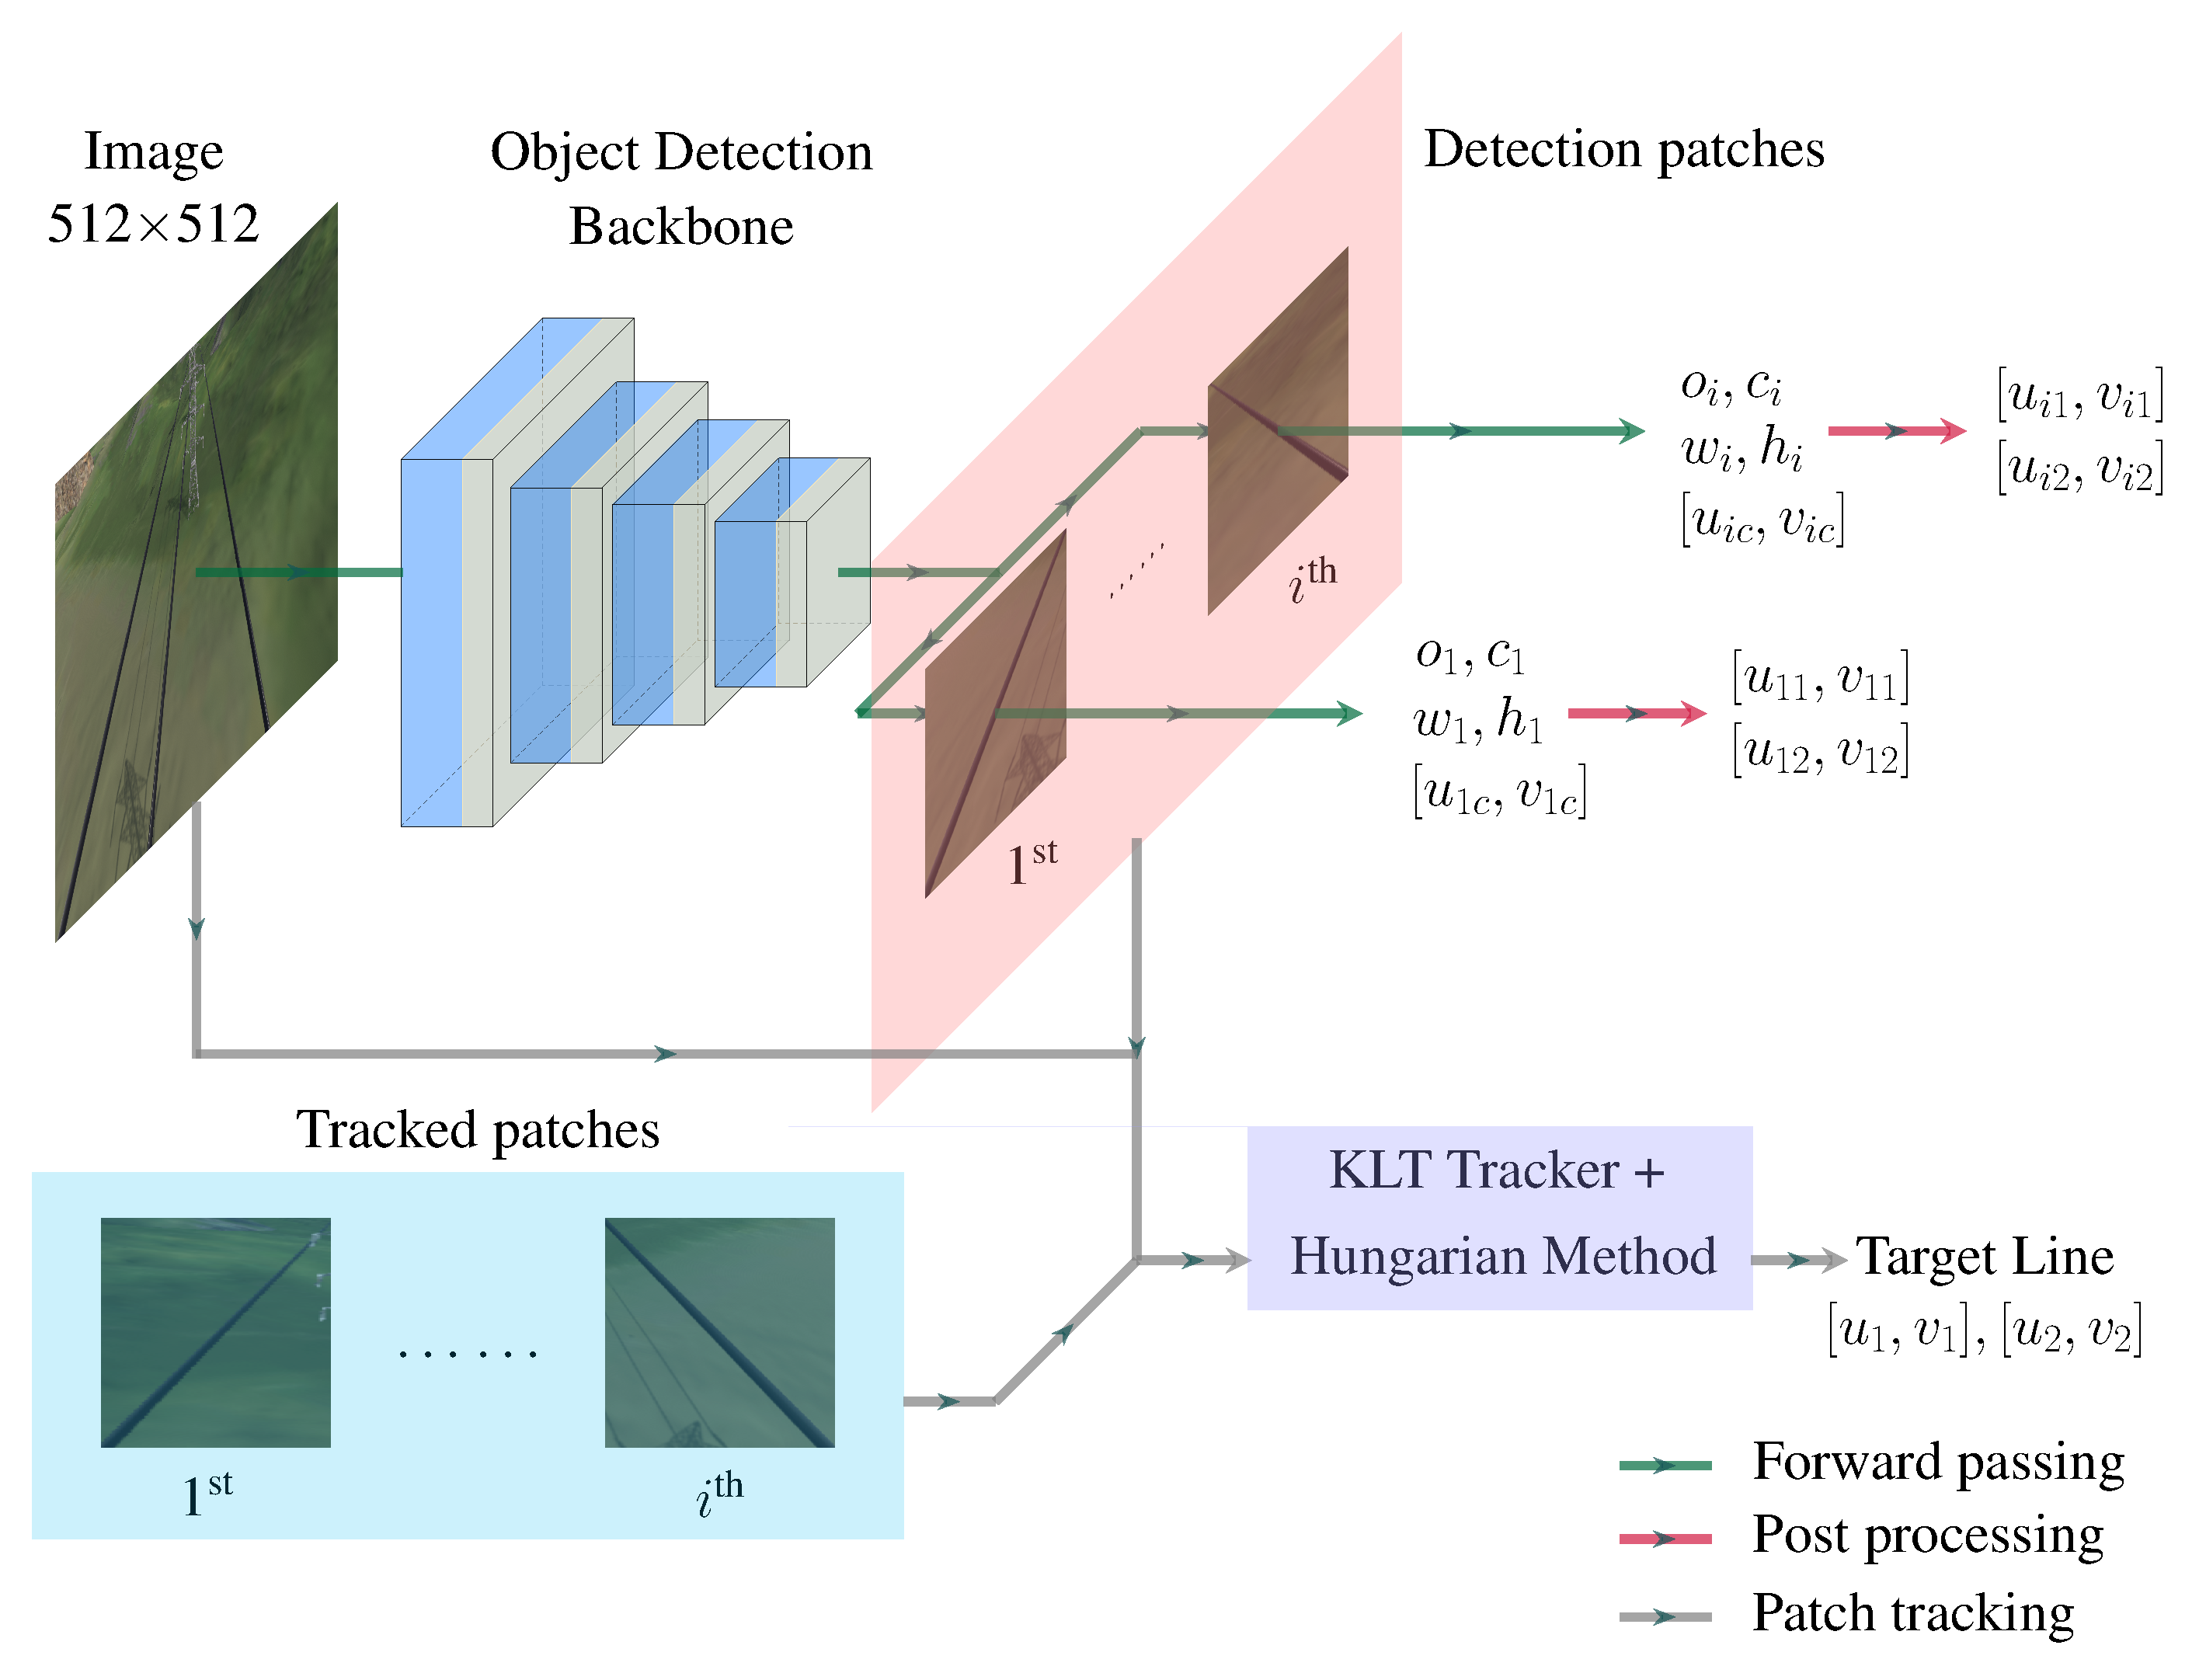
\includegraphics[width=\columnwidth]{figures/framework.pdf}
    \caption{ \iros{Overview of our learning-based power line detector and tracker. The detector takes a single RGB image as input and outputs end points of the detected power lines in pixel coordinates. The center patch of each detection is matched with the prediction of the previous patch using the Hungarian method~\cite{kuhn1955hungarian}. We use a KLT tracker~\cite{lucas1981iterative} to perform tracking. The final output is the tracked lines endpoints which are given to the MPC.}}
    \label{fig:perception}
    \vspace{-1.5ex}
\end{figure}
\iros{ As shown in Fig.~\ref{fig:perception}, our detector takes monocular RGB images as input and outputs: (i) width $w_i$ and height $w_i$ of the bounding boxes that fully contain the detected power line, where $i$ indicates the number of detection; (ii) the inclination of the line $o_i$ (either +1 or -1). The endpoints of positive inclined lines, i.e., $o_i=+1$, correspond to the top-left and bottom-right corners of the bounding box. The endpoints of negative inclined lines correspond to the top-right and bottom-left corners of the bounding box; (iii) the center of the line $[u_{ic}, v_{ic}]$; (iv) the confidence score $c$ of the prediction. If the confidence score is not larger than a predefined threshold (we use 0.8 in all our experiments), the detection is labeled as invalid and is not used. To perform tracking, we use a tracking-by-detection approach to track the detected power lines.} In the first step, we track the center patch of the detected bounding box, of dimension 25$\times$25 pix, using a 4 layers Lukas-Kanade tracker (KLT)]~\cite{lucas1981iterative}. In the second step, we compute the similarity score between bounding boxes in two consecutive frames as the sum of the KLT error and the area difference between the two bounding boxes normalized by the image size. In the final step, we find the best matches using the Hungarian method~\cite{kuhn1955hungarian}. The final outputs are the endpoints of the tracked line in the pixel coordinate $[u_1, v_1], [u_2, v_2]$. Then we transform the endpoints, incorporating depth detection and state estimation, into the world frame to derive $\bm{p}_{W{L_1}}, \bm{p}_{W{L_2}}$.
% These values are then integrated into our MPC. in~\ref{eq:line_endpoints_camera_frame}.

Among the datasets which contain power lines~\cite{zhang2019detecting, abdelfattah2020ttpla}, there is a limited amount of labeled data and scene variability. Consequently, they are not suitable for training a robust power line detector. For this reason, we created a new dataset for power line detection based on the photo-realistic simulator Flightmare~\cite{song2021flightmare}. We collected a dataset of $\sim$30k images of labeled power lines of different colors and thicknesses in different 6 environments (c.f. Fig.~\ref{fig:scenes}). The dataset is split into training (80\%), validation (10\%), and test  (10\%) sequences. We train our power line detector on the training sequence and use the validation sequence for hyperparameters tuning.

\iros{Our current approach requires that the user specifies which power line to track, e.g., the ID $i$ from the detection. The ID cannot be changed during the flight. We leave as part of future work the extension of the MPC formulation to track different lines. A current limitation of the line tracked is the missing information on the temporal history of the lines. If a power line is not tracked between two frames, the detector is unable to continue tracking the previous line. To address this issue, a possible solution would be to implement a hibernation mechanism as in~\cite{dietsche2021powerline}.}

%
\begin{figure}[t!]
    \centering
    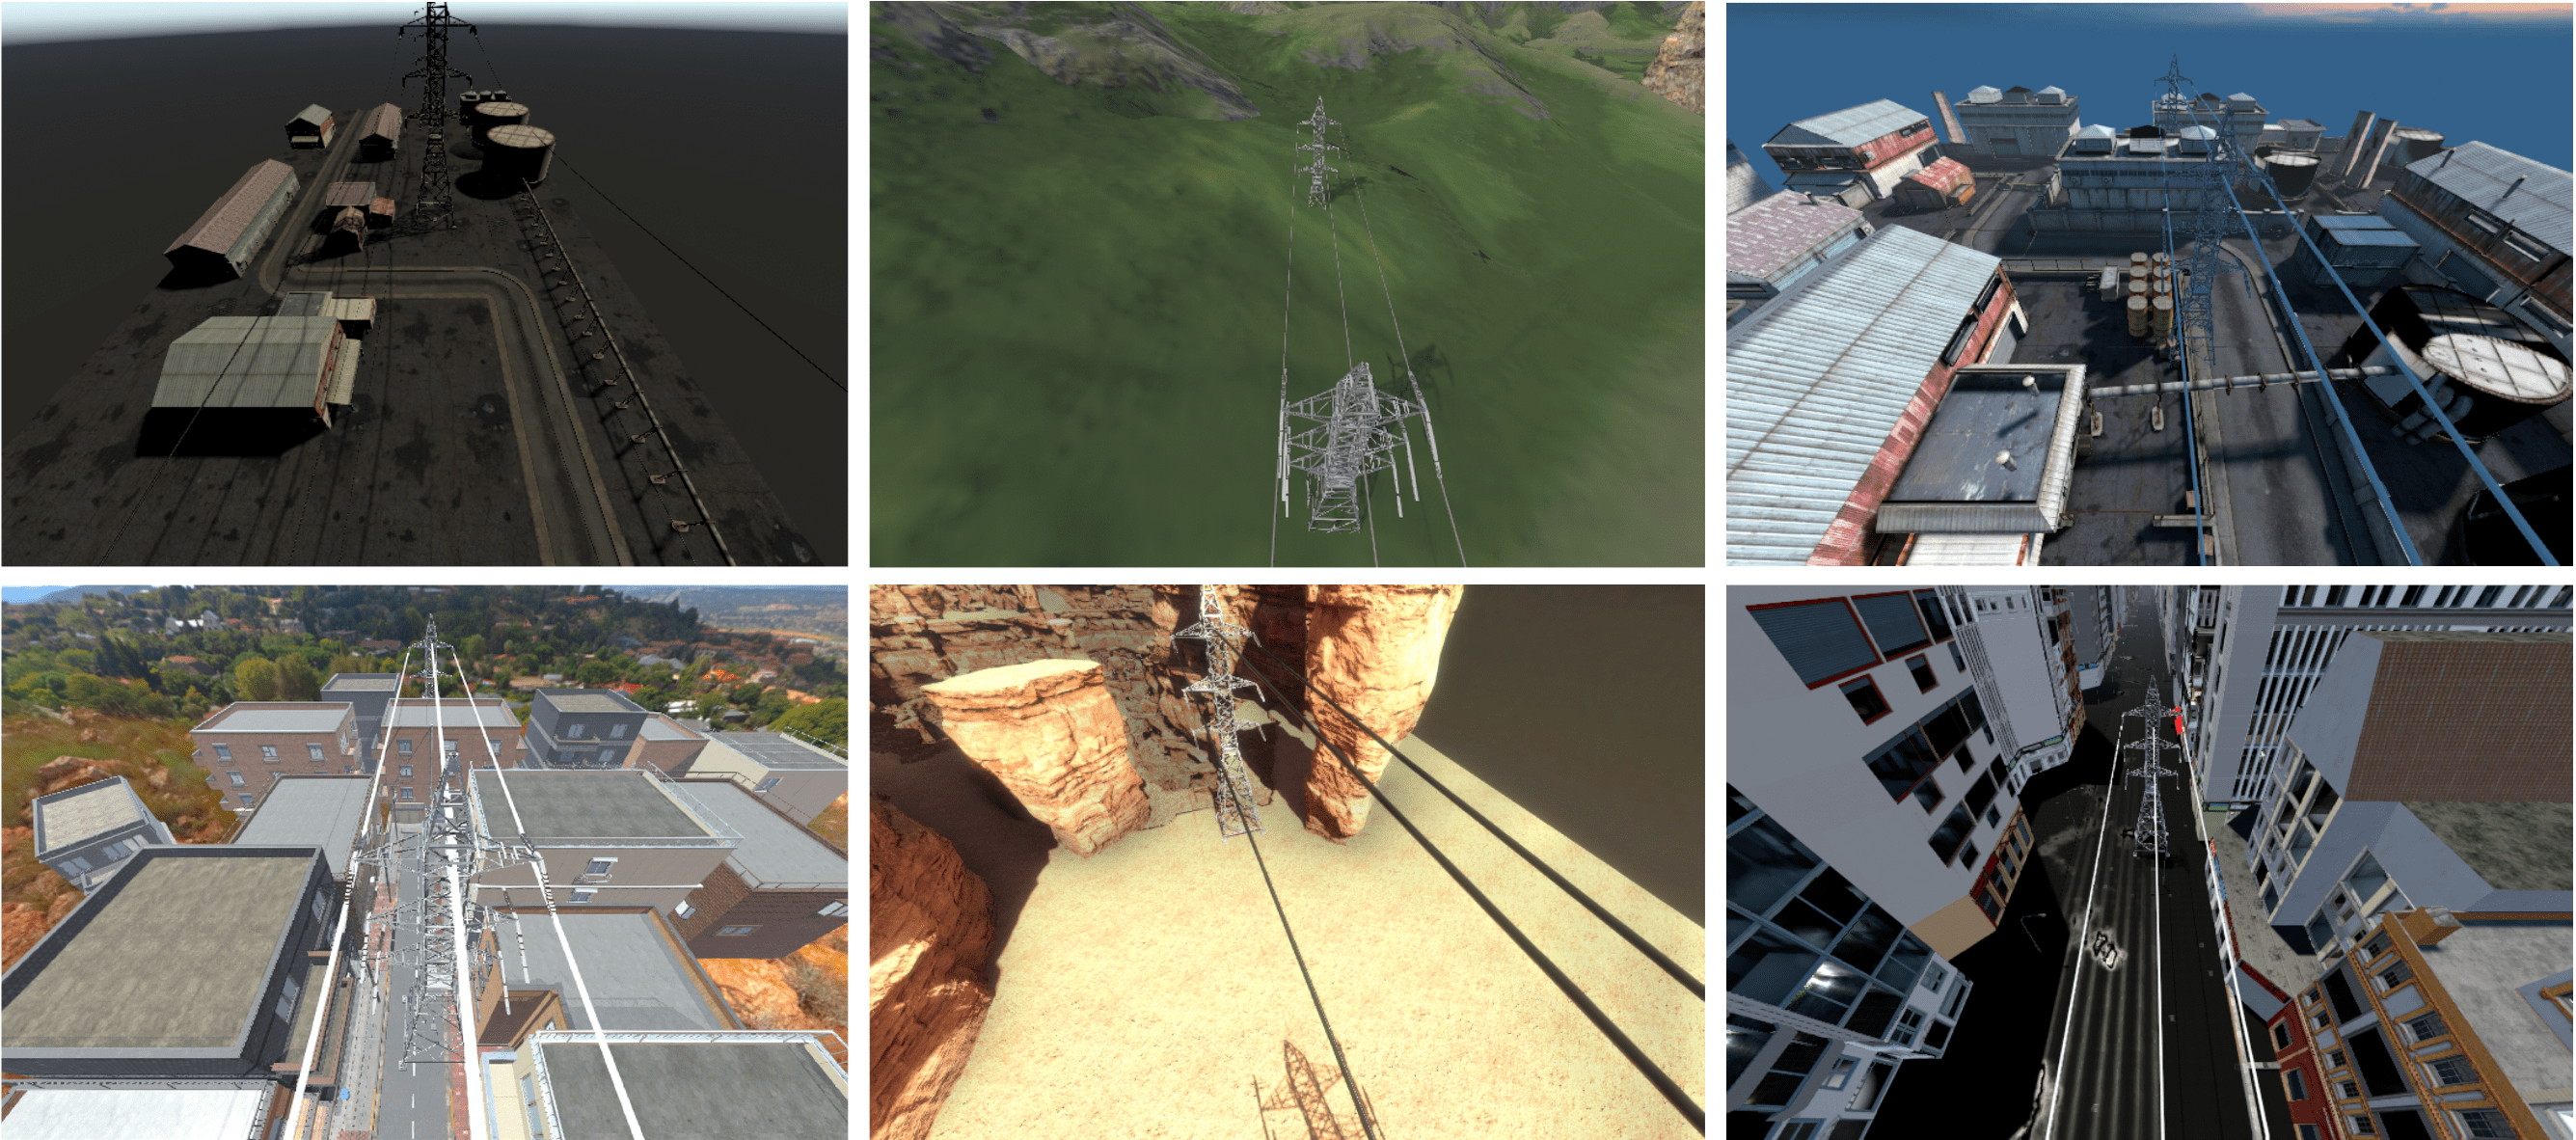
\includegraphics[ width=0.95\columnwidth]{figures/scenes_comp.png}
    \vspace{0.5ex}
    \caption{Sample images from the proposed power line dataset.}
    \label{fig:scenes}
    \vspace{-1.5ex}
\end{figure}

\subsection{Obstacle Detection}
We use ellipsoids with constant but unknown sizes to represent obstacles. The state of an obstacle is defined as $\left(\bm{p}_{WO}, a_o, b_o, c_o\right)$, which contains the position of the center of the ellipsoid in the world frame and the length of its semi-principal axes. Our obstacle detection module is based on U- and V- disparity maps as proposed in~\cite{oleynikova2015reactive}. The U-map is a histogram of disparity values accumulated over the columns of the image. The V-map is a histogram of disparity values accumulated over the rows of the image. These disparity maps are used to detect obstacles from depth images.
